
\RequirePackage{fix-cm}
\documentclass[]{rsos}%%%%where rsos is the template name

%% *** Do not adjust lengths that control margins, column widths, etc. ***
\usepackage{subfigure}
\usepackage{lineno}
\begin{document}

% \linenumbers
%%%% Article title to be placed here
\title{Insert the article title here}

\author{%%%% Author details
Alasdair D. F. Clarke$^1$, Jessica L Irons$^2$, Warren James$^3$, Andrew B Leber$^2$ and Amelia R Hunt$^3$}

%%%%%%%%% Insert author address here
\address{$^{1}$Department of Psychology, University of Essex, Colchester, UK\\
$^{2}$Department of Psychology, The Ohio State University, Columbus, USA\\
$^{3}$School of Psychology, University of Aberdeen, Aberdeen, UK}

%%%% Subject entries to be placed here %%%%
\subject{Behaviour, evolution}

%%%% Keyword entries to be placed here %%%%
\keywords{visual search, optimal behaviour, eye movements}

%%%% Insert corresponding author and its email address}
\corres{Alasdair Clarke\\
\email{a.clarke@essex.ac.uk}}

\begin{abstract}
Some abstract goes here
\end{abstract}

%%%%%%%%%% Insert the texts which can accomdate on firstpage in the tag "fmtext" %%%%%

\begin{fmtext}
%%%%%%%%%%%%%%%%%%%%%%%%%%%%
\section{Introduction}
%%%%%%%%%%%%%%%%%%%%%%%%%%%%

As is common in cognitive psychology, most visual search literature has focused on how the average participant performs in the task, despite it being well known that there is a great deal of variability between one subject and the next. From Treisman's work on Feature Integration Theory\cite{treisman1980} to the latest incarnation of the Guided Search Model\cite{wolfe2015}, we now have a good understanding of what makes some search targets effortless to find, while others require careful inspection. However, these theories and models have neglected the question of why some observers find visual search so much harder than others. These differences can emerge from several different sources of variation: tiredness\cite{mackworth1948}, information-processing ability, speed-accuracy trade-off, motivation, visual impairments\cite{nowakowska2016}, and search strategies\cite{boot2006}. Although their existence has previously been noted\cite{mackworth1948}, a rigorous examination of individual differences in visual search is a challenge that has not been taken up by many researchers, and questions about their importance and stability remain relatively under explored. 

In the current study, we focus on one source of individual differences in visual search: strategy. By search strategies, we refer to a collection of behaviours that all observers can freely choose from when they search a display. Examples include choosing to adopt a systematic left-to-right and top-to-bottom strategy\cite{gilchrist2006}, or the type of guided search behaviour in which locations that are more likely to contain the target are prioritised\cite{wolfe2015}. 
\end{fmtext}
\maketitle
\twocolumn
A striking example of the effect of strategy is given by Boot and colleagues\cite{boot2006}. They asked participants to monitor a cluttered display for an object changing colour or suddenly appearing. Large individual differences were found with respect to the number of saccades participants made while monitoring the stimulus, and this was negatively correlated with detection performance. Proulx\cite{proulx2011} demonstrated that participants differed in how they prioritised visual features (color or orientation) when searching through a set of objects for one with a particular color-orientation combination. These differences in search strategy explained some of the variation in the extent to which participants were distracted by an irrelevant object of a unique size. However, participants were largely unaware of the search strategy they employed, and the majority were unable, or unwilling, to comply with instructions to employ a particular strategy.

Eye movement strategies have also been shown to be an important source of individual differences in visual search efficiency. Nowakowska, Clarke \& Hunt\cite{nowakowska2017} designed a simple search paradigm to discriminate between optimal\cite{najemnik-geisler2008} and stochastic \cite{clarke2016} search strategies. The task involved searching through arrays of line segments arranged such that those on one side of the display all had a very similar orientation ("homogeneous"), while those on the other side had higher variance ("heterogeneous", see Figure \ref{fig:exampleStimuli} for an example). This meant that targets appearing on the homogeneous side would be highly salient, and targets on the heterogeneous side  would be much harder to find. With these stimuli, the optimal eye movement strategy is to only search the heterogeneous half , as targets on the homogeneous side can be detected with peripheral vision. We will refer to this paradigm here as the Split-Half Line Segment task (SHLS). While some participants initially searched the displays near optimally, others carried out strategies counter to this, failing to even match the performance of the stochastic searcher. Furthermore, the degree to which they made saccades in line with the optimal search strategy was strongly correlated with their reaction times. A related version of this paradigm has been used in research investigating eye movement strategies in response to (simulated) hemianopia\cite{nowakowska2016,nowakowska2018}, with similar conclusions: the full spectrum of individual differences in strategy was observed, from near-optimal to the opposite of optimal. It is therefore not possible to conclude whether optimal or stochastic models better describe search without first explaining individual variablility.

A similar range of strategies, from random to near-optimal, has been found by Irons \& Leber with the Adaptive Choice Visual Search (ACVS) paradigm\cite{irons-leber2016}, designed to explore how feature-based attention is used. This paradigm involves stimuli made up of small coloured boxes (red, blue, green and a fourth colour that varies from red, through purple, to blue and back again) with numerals written inside them (See Figure \ref{fig:exampleStimuli}). The target is a defined as a red or blue box with a numeral between 1 and 4, and on each trial one target of each colour is present. The participant's task is to find one of either target as quickly as possible and report the numeral. On trials in which the fourth colour is red (or close to red), participants should search through the blue boxes and report the blue target, as there will be fewer distracters. As the fourth colour changes to through purple to blue, participants should update their strategy and search for the red target. The results showed that participants varied substantially along two key dimensions: how frequently they used the more effective target color to search (varying from chance performance to near optimal), and how often they changed between colours. Further work has shown that these differences are stable over time (between one and ten days) with test-retest correlations of around $r \approx 0.8$\cite{irons-leber2018}.

\begin{figure*}
\centering
\subfigure[][]{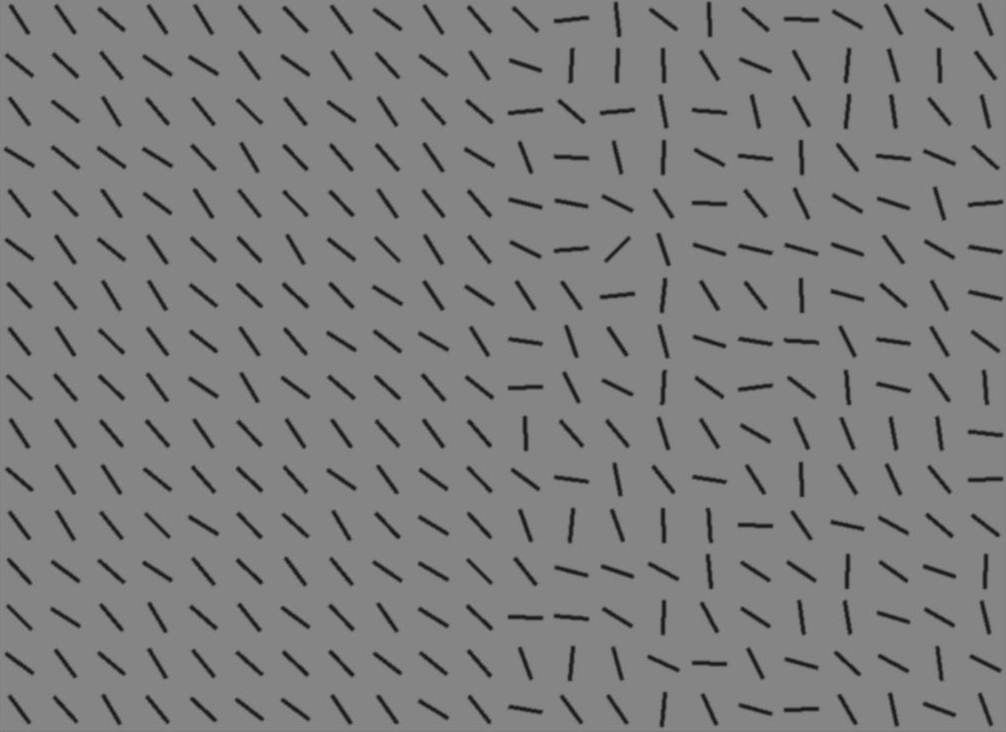
\includegraphics[height=3cm]{figures/split-half.png}}
\subfigure[][]{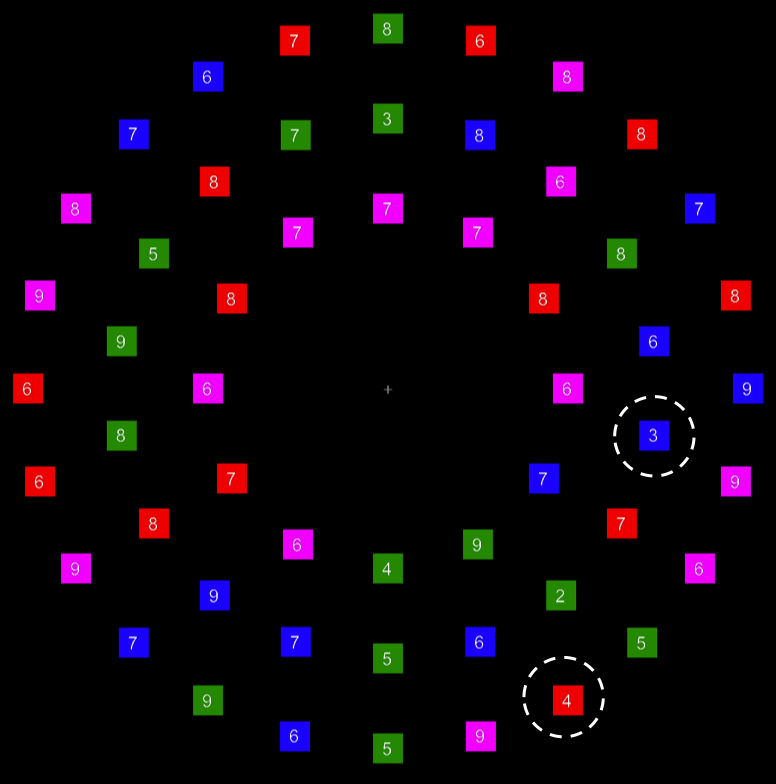
\includegraphics[height=3cm]{figures/adaptive.png}}
\subfigure[][]{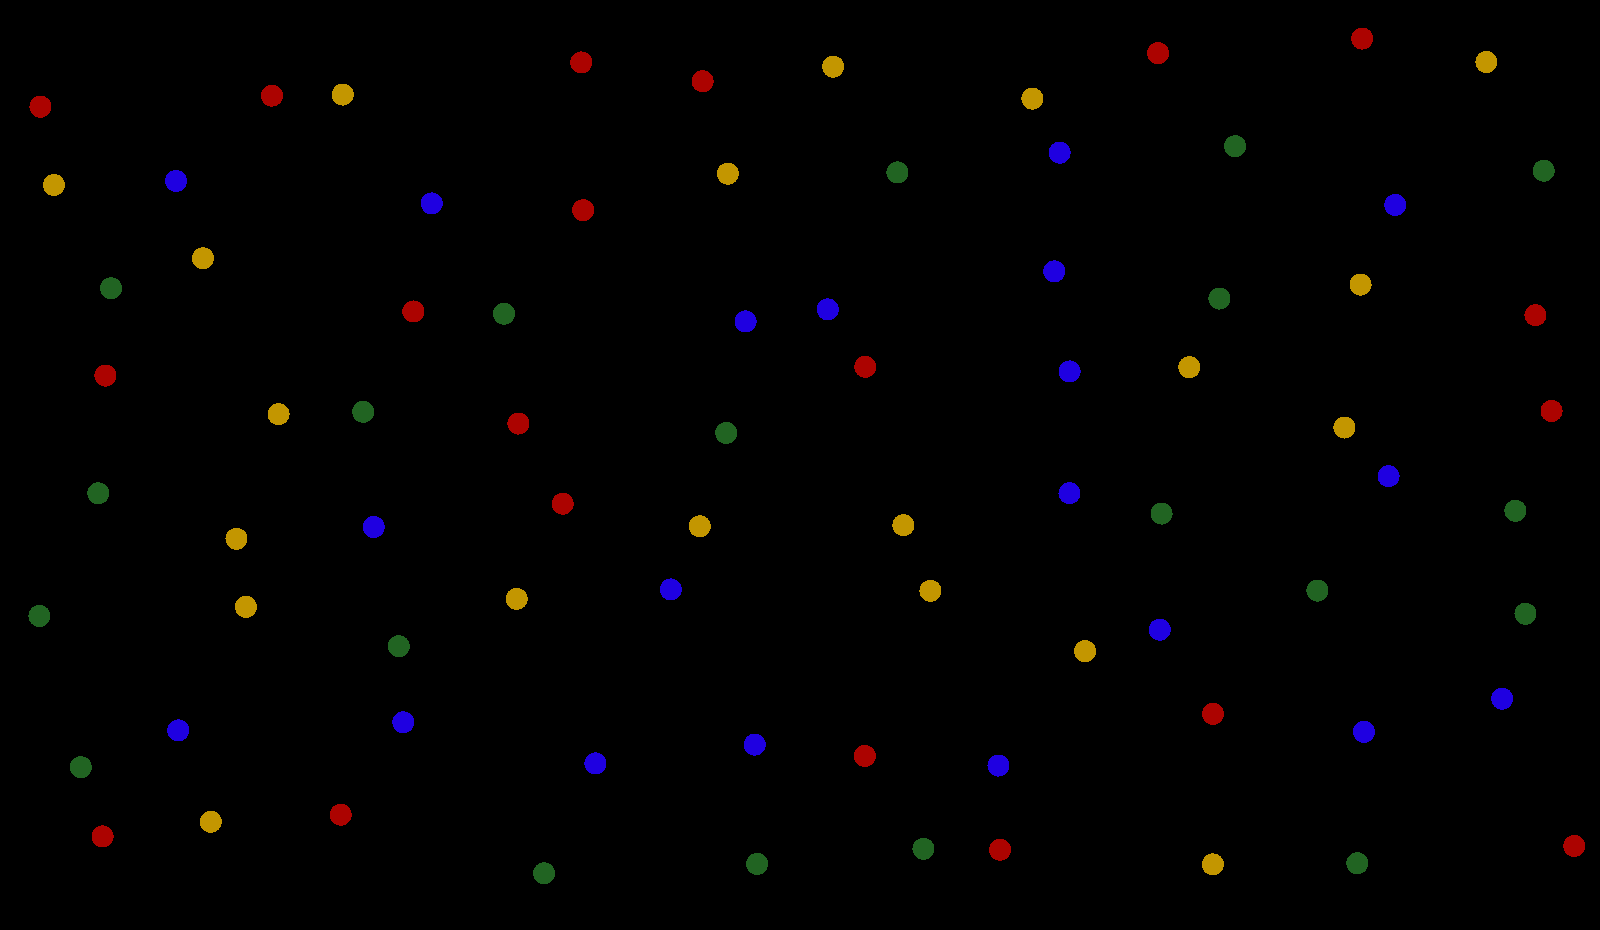
\includegraphics[height=3cm]{figures/foraging.png}}
\caption{Example stimulus from the (a) \textit{split-half}, (b) \textit{adaptive choice} and (c) \textit{foraging} paradigms.}
\label{fig:exampleStimuli}
\end{figure*}

<<<<<<< HEAD
Another example of differences in search strategy comes from the foraging literature \cite{kristjansson2014,johannesson2016}. In this context, foraging is a visual search task in which there are multiple targets on each trial. Participants were asked to search through a set of items from four categories, with two categories classed as targets. In the conjunction condition (searching for red-horizontal and green-vertical line segments among red-vertical and green-horizontal distracters), most observers searched in runs, finding all the targets of one target category, and then switching and finding the targets in the other category. This strategy has previously been observers in animal foraging \cite{dawkins1971}, and suggests holding one complex target tenplate in mind at a time is a better strategy than switching templates. However, a sub-set of observers, termed `super-foragers', were able to change between search target categories with no cost to performance. This study has been run on touch displays\cite{kristjansson2014} (observers are asked to tap on as many targets as they can as quickly as possible) and a 3D computer game (in which participants navigate a squirrel through a virtual environment picking up targets with different feature combinations)[IN PREP], with super-foragers present in both versions. While test-retest reliability has not been measured explicitly for the foraging paradigm, the task was used as a measure to assess the effect of a six day long mindfulness retreat on cognitive performance\cite{hartkamp2017}. From a re-analysis of these data, we can estimate that the test-retest reliability is $r \approx 0.7$ for the feature condition and $r \approx 0.88$ for the conjunction search.  
%is this r correlating reaction time, or switching?
=======
Another example of differences in search strategy comes from the foraging literature \cite{kristjansson2014,johannesson2016}. In this context, foraging is a visual search task in which there are multiple targets on each trial. Participants were asked to search through a set of items from four categories, two of which were classed as targets. In the conjunction condition (i.e. searching for red-horizontal and green-vertical line segments among red-vertical and green-horizontal distracters), most observers searched in runs of one target category or another. This strategy has previously been observers in animal foraging literature \cite{dawkins1971}. However, a sub-set of observers, termed `super-foragers' showed no switch cost. This study has been run on touch displays\cite{kristjansson2014} (observers are asked to tap on as many targets as they can as quickly as possible) and a 3D computer game (in which participants navigate a squirrel through a virtual environment picking up targets with different feature combinations)[IN PREP], with super-foragers present in both versions. While test-retest reliability has not been measured explicitly for the foraging paradigm, the task was used as a measure to assess the effect of a six day long mindfulness retreat on cognitive performance\cite{hartkamp2017}. From a re-analysis of these data, we can estimate that test-retest reliability for the mean lengths of runs is $r\approx 0.88$.
>>>>>>> origin/master

Previous research has investigated the relationship between these behaviours to \hyphenation{psychometric} measures, but to date, these differences have not shown strong correlations with other attributes. In the ACVS paradigm, Irons \& Leber found no evidence of a correlation between the proportion of optimal choices made by observers and measures of visual working memory or trait compulsivity\cite{irons-leber2016}. Similarly, the differences foraging behaviour are not accounted for by working memory or inhibitory control\cite{johannesson2017}. 

A common theme emerging from these studies is the observation that individual strategies vary in their degree of effectiveness or optimality. However, ``visual search'' encompasses a wide range of specific tasks, each tapping into a different aspect of behaviour (e.g. feature-based attention, information sampling). The aim of the present study is to investigate the extent to which individual differences are stable across different visual search paradigms. Are observers who use the optimal strategy in the SHLS paradigm also more optimal in the ACVS task? Does it make sense to talk about `super-searchers' who show above average performance in a range of search tasks (analogous to the 'super-recognizers' of the face-recognition literature \cite{russell2009}? Are the super-foragers consistently better or worse than more typical searchers in the other two paradigms? As a secondary question, we will measure the test-retest reliability of the differences found in the SHLS paradigm. 

%%%%%%%%%%%%%%%%%%%%%%%%%%%%%%%%%%%%%%%%%%%%%%%%%%%%%%%%
\section{Methods}
%%%%%%%%%%%%%%%%%%%%%%%%%%%%%%%%%%%%%%%%%%%%%%%%%%%%%%%%

The methods and planned analysis for this study were registered on the Open Science Framework\footnote{insert URL} before data collection started.

\subsection{Participants}
64 students from the University of Aberdeen took part in this study. Participants were compensated for their time with either  course credit or \pounds 15. All participants will sign a form giving informed consent. The study was approved by the University of Aberdeen Psychology Ethics Committee. 

Sample size was determined in part by a power analysis, and in part due to constraints with counter-balancing. $n = 64$ participants means we should be able to detect correlations with $r > 0.34$ with $\alpha = 0.05$, $\beta = 0.80$ between the different visual search paradigms. The sample size is therefore of sufficient size to detect relatively small correlations.

\subsection{Materials and Procedures}

The study consists of three paradigms from the visual search literature in which large individual differences have been  found\cite{nowakowska2017, irons-leber2016, kristjansson2014}. Example stimuli can be seen in Figure \ref{fig:exampleStimuli}. A brief overview of each paradigm is given below, with full details in \textit{supplementary materials}. The three tasks will be completed over two sessions, approximately one week apart. The SHLS was run in both sessions allowing us to measure test-retest reliability. The order in which participants completed the tasks was counter-balanced. There are 16 different possible orders of tasks/conditions; four participants completed each order for a total of 64.

The display was presented on a 17-inch CRT monitor with a resolution of $1400 \times 1050$. Stimulus generation, presentation and data collection were controlled by MATLAB and the psychophysics and eyelink toolboxes \cite{brainard1997,cornelissen2002} run on a Powermac. 

\subsubsection{Split-half Line Segments}

Stimuli consisted of arrays of black oriented line segments against a grey background. Each line segment had a length of $\approx$$1.6^{\circ}$ of visual angle irrespective of screen resolution. The target was oriented $45^{\circ}$ clockwise, while the distractor items had a random orientation with a mean of $45^{\circ}$ anti-clockwise. The variance was low ($18^{\circ}$) on one half of the display to create a homogeneous texture, and high ($95^{\circ}$) on the other side to create a heterogeneous texture. This means that when the target is present on the homogeneous side of the stimulus, it can be easily be detected with peripheral vision, but when it is in the heterogeneous half, it is much harder to detect. This was verified in a pilot experiment reported in \cite{nowakowska2017}.  There were a total of 160 trials and homo- and heterogeneous sides of the display were randomly varied from trial to trial. The position of the dominant eye was recorded using a desktop-mounted EyeLink 1000 eye tracker (SR Research, Canada). 

This paradigm was carried out twice, once in each testing session, to give us an estimate of how consistent participants are in their search strategy over time. 


\subsubsection{Adaptive Choice Visual Search}

The ACVS was based on the task described in \cite{irons-leber2016}, Experiment 1. Each search display was composed of 54 small squares arranged in three concentric rings around fixation, with 12, 18 and 24 items in the inner, middle and outer rings respectively. The same screen was used as in the Split-half Array Search, however, due to changes of screen resolution, the size of the squares changed. Participants sat $\approx 47$cm from the screen. Of the 54 squares, 13 were red, 13 were blue, 14 were green and 14 were "variable". Variable distractors change colours from trial-to-trial according to a 24 trial cyclical pattern: the distractors would be red for five trials (called a "red plateau"), then across a period of seven trials, they would change colour from almost red to magenta (at the fourth trial in the transition) to almost blue. The variable distractor would then be blue for five trials (blue plateau), and then transition back from almost blue through magenta to almost red. 

A white digit appeared inside each square. Two targets - a red square and a blue square each with a digit between 2 and 5 - were embedded in every search display. The two target digits were always different, to enable us to distinguish the chosen target. The remaining red, blue and variable squares all contained digits between 6-9. Green squares could contain any digit between 2-9. The location of the targets and distractor within the search display were randomized on each trial.

Participants were informed that the search displays would contain two targets on every trial, that they need only find one target on each trial and that they were always free to search for either one.   

\subsubsection{Mouse Click Foraging Task}

The foraging task (MCFT) was based on \cite{kristjansson2014} and \cite{johannesson2016} except that we used a mouse clicks to register responses rather than a touchpad. 

In the feature foraging task, search displays contained 80 small circles, 20 red, 20 green, 20 blue  and 20 yellow. Stimuli were arranged in a $10 \times 8$ grid, but the position of each item within the grid space was jittered to create a more random spatial arrangement. The location of item colours to grid locations was completely randomized. For half of the participants, targets were red and green circles, and for the other half of participants, targets were blue and yellow circles. Participants were asked to collect all of the targets within a trial by using the mouse to click on each target. Clicking on a target caused it to disappear from the display. If the participant clicked erroneously on a non-target, the trial immediately ended and a replacement trial was begun. In the conjunction foraging task, search displays were composed of both circles and squares. For half of the participants, the shapes were red and green (equal numbers of red circles, red squares, green circles and green squares), and for the remaining participants the shapes were blue and yellow. Targets were defined by conjunctions of colour and shape (e.g., red squares and green circles, with red circles and green squares as distractors). The assignment of targets and distractors was assigned at random for each participant. The procedure was otherwise identical to the feature foraging task. 

%%%%%%%%%%%%%%%%%%%%%%%%%%%%%%%%%%%%%%%%%%%%%%%%%%%%%%%%%%%%%%%%%%%%%%%%%%%%%%%%%%%%
\section{Results}
%%%%%%%%%%%%%%%%%%%%%%%%%%%%%%%%%%%%%%%%%%%%%%%%%%%%%%%%%%%%%%%%%%%%%%%%%%%%%%%%%%%%

\subsection{Replication of each paradigm}

\subsubsection{Split-half Line Segments}

Our results are consistent with the original SHLS study\cite{nowakowska2017}. Only trials with a correct target absent/present response were included in the analysis. Some participants performed exceptionally poorly and were removed from further analysis\footnote{Full details given in the \textit{supplementary materials}}. All reaction times were $\log_2$ transformed. In order to characterise each participant's behaviour in this task, we will compute the proportion of the first $n$ fixations that were on the heterogeneous (difficult) side of the stimuli, over all correct target absent trials. Previous work\cite{nowakowska2017} demonstrated a strong correlation between this metric (for $n=5$) and reaction times ($r=.93$).

The correlation between accuracy and reaction times between the two sessions is shown in Figure \ref{fig:splithalf_summary}(a, b). We can clearly see that there are large differences from one participant to the next in terms of both the proportion of hard targets found, and reaction times. Furthermore, test-retest reliability appears to be reasonable, with Pearson's $r \in [0.71, 0.89]$ ($95\%$ confidence interval) for accuracy in finding targets on the hard heterogeneous half of the display. We get similar scores for the correlation in reaction times between sessions \textit{a} and \textit{b} for heterogeneous targets, ($r \in [0.54-0.81]$), homogeneous targets ($r \in [0.52-0.80]$) and target absent ($r \in [0.66-0.86]$). The reduced correlation for the homogeneous targets is likely due to the restricted range.

\begin{figure}
\centering
\subfigure[][]{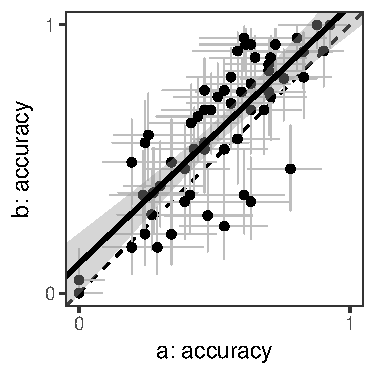
\includegraphics[width=3.25cm]{../Scripts/lineseg/scratch/acc_correlation.pdf}}
\subfigure[][]{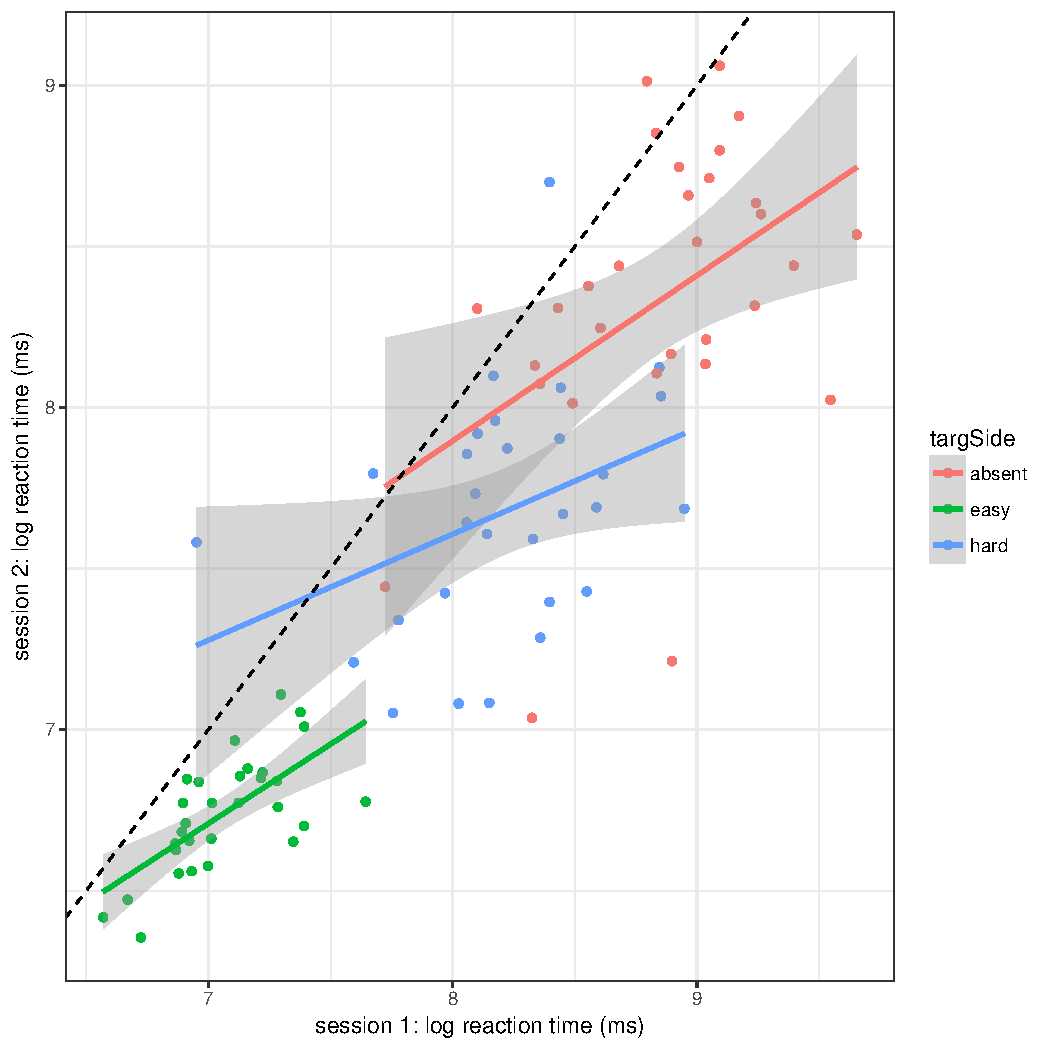
\includegraphics[width=3.25cm]{../Scripts/lineseg/scratch/rt_correlation.pdf}}
\subfigure[][]{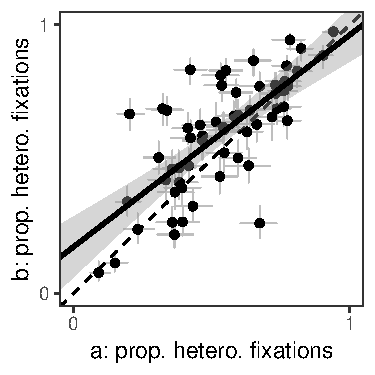
\includegraphics[width=3.25cm]{../Scripts/lineseg/scratch/strat_corr.pdf}}
\subfigure[][]{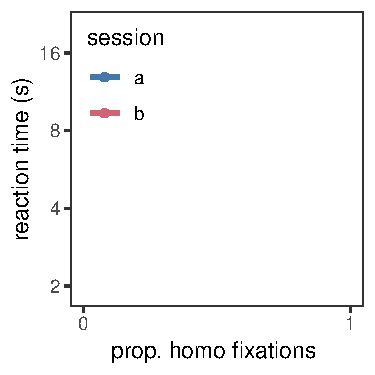
\includegraphics[width=3.25cm]{../Scripts/lineseg/scratch/strat_compare_meanlog_rt.pdf}}
\caption{Each point represents a participant and the error-bars indicate 95\% confidence intervals. Correlation between the two sessions of the SHLS paradigm for (a)  accuracy (TP-heterogeneous trials only); (b) reaction times and (c) search strategy (TA trials only). (d) Initial search strategy correlates with reaction times in both sessions. }
\label{fig:splithalf_summary}
\end{figure}

We can also look at the initial search strategies adopted by our participants \ref{fig:splithalf_summary}(c, d). Again, we see large and stable individual differences across the two sessions (test-retest $r \in [0.63, 0.86]$ for the proportion of the first five saccades to the heterogeneous half of the display for target absent trials). More importantly, as with \cite{nowakowska2017}, we see that the search strategies give a good correlation with reaction times in both session a, $r \in [0.52, 0.82]$ and session b, $r \in [0.50, 0.80]$.


\subsubsection{Adaptive Choice Visual Search}

Participants with accuracy more than 3 SD below the group mean were excluded from analyses. For RT analyses, trials with RTs less than 300ms or more than 3 SD about the participant's mean were excluded. 

Two measures of individual strategy use were used: 1) Optimal choices, defined as percent of plateau trials in which the individual chose the optimal target (i.e., the target with the fewest distractors. When the variable distractor was red, the optimal choice was blue, and vice versa), and 2) Switch rate, the percent of trials in which the individual switched target colour (i.e., the colour chosen on trial $N$ was different to the colour chosen on trial $N-1$).  


The results for the ACVS were consistent with previous findings \cite{irons-leber2016,irons-leber2018}. We can clearly see from figure \ref{fig:acvs_summary} that there are individual differences in both the proportion of optimal targets reported (range $33.62\%$ - $97.50\%$, $M = 56.99$, $SD = 14.75$) and switch rate (range = $0\% - 56.68\%$, $M = 28.46$, $SD = 13.54$). 

\begin{figure}
\centering
\subfigure[][]{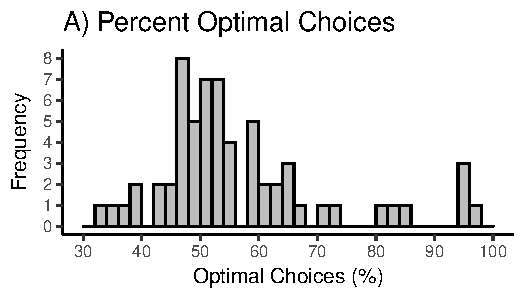
\includegraphics[width=6.5cm]{../Scripts/adaptchoice/ac_percentOpt_hist.pdf}}
\subfigure[][]{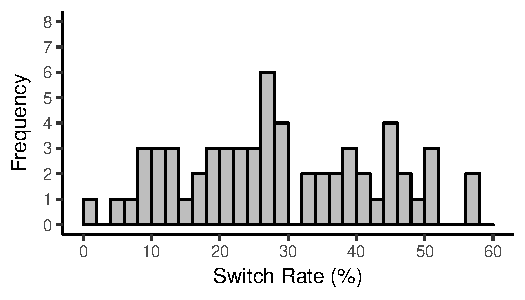
\includegraphics[width=6.5cm]{../Scripts/adaptchoice/ac_switchRate_hist.pdf}}
\caption{Histograms showing the range of individual differences found in the ACVS task.}
\label{fig:acvs_summary}
\end{figure}

\subsubsection{Mouse Click Foraging Task}

Only completed, accurate trials were analysed. RTs were defined across the entire trial (i.e., from the start of the trial until the final target was collected). The main measure of interest was average run length per trial. A run was defined as a succession of one or more of the same target type, which was followed and preceded by the other target or no target. The average run length was the average number of target selections in a run. 

The multiple-target foraging results were also in line previous findings \cite{kristjansson2014,johannesson2016}. As expected, run lengths were shorter for feature foraging ($M = 3.24$, $SD = 3.19$) than conjunction foraging ($M = 10.64$, $SD = 7.01$), $t(55) = 8.03$, $p < .001$ (PREFER DIFFERENT STATS HERE? CI [-9.25,-5.55]) suggesting more frequent foraging for multiple targets concurrently when those targets were defined by features than by conjunctions. However, both showed significant individual variation: Feature run length varied between 1.87 and 20, and conjunction run length varied between 1.00 and 19.67. Figure \ref{fig:foraging_summary} depicts run length across the trials separately for each individual. Twenty ``super-searchers'' were revealed, identified by short run lengths for both feature and conjunction targets. 

\begin{figure}
\centering
\subfigure[][]{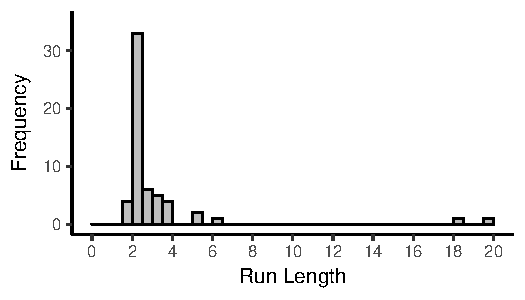
\includegraphics[width=6.5cm]{../Scripts/foraging/fg_featureRunLength_hist.pdf}}
\subfigure[][]{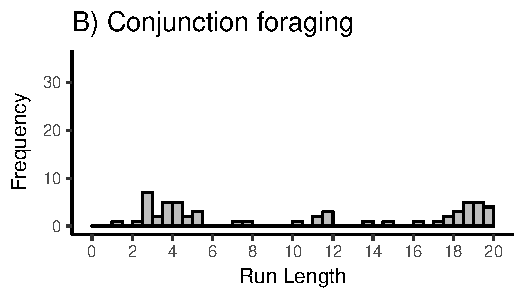
\includegraphics[width=6.5cm]{../Scripts/foraging/fg_conjRunLength_hist.pdf}}
\caption{Histogram of mean run lengths for (a) feature and (b) conjunction foraging tasks.}
\label{fig:foraging_summary}
\end{figure}

\subsection{Correlations Between Paradigms}

The results above demonstrate that we have successfully replicated the previous findings around individual differences in visual search strategy in each of the three paradigms. Furthermore, the split-half paradigm has a test-retest reliability of $r \in [0.65. 0.86]$, similar to that of the ACVS task ($r \in [0.72, 0.9]$), suggesting that the strategies different individuals chose to use in each of these tasks are somewhat stable. Given this, we now investigate the extent to which an individual's performance in one of the tasks tells us about how well they will do in the other two. 

The feature search condition from the MCFT will be discarded from this analysis, as the individual differences of interest relate to how people search in the conjunction condition. Measures for the SHLS task will be taken from 


The results presented in Figure \ref{fig:all_the_cor} convincingly demonstrate that there are no strong correlations between any of the strategies chosen by observers in SHLS, ACVS and MCFT tasks \footnote{More comparisons are presented in the \textit{supplementary materials.}}. 
While there is no indication of a relationship between strategies across the different paradigms, perhaps there is still a correlation between the reaction times due to some participants having higher levels of motivation than others, or stable speed-accuracy trade-offs between the different tasks. Differences relating to their information-processing speed and their ability to ignore distractors would also play in to such a correlation. However, as with search strategy, we again find all the correlations to be weak, typically $0.27 < r <0.30$ but positive (Figure \ref{fig:all_the_cor}). None of these correlations are statistically significant ($p>0.05$). Even if we optimistically take all the data together as suggesting a robust correlation in reaction times from paradigm to paradigm, the upper bound of $r=0.30$ means that this correlation only accounts for at best $10\%$\footnote{i.e., $R^2 = 0.3^2 = 0.09$} an individual's performance. 

% \begin{figure}
% \centering
% \subfigure[][]{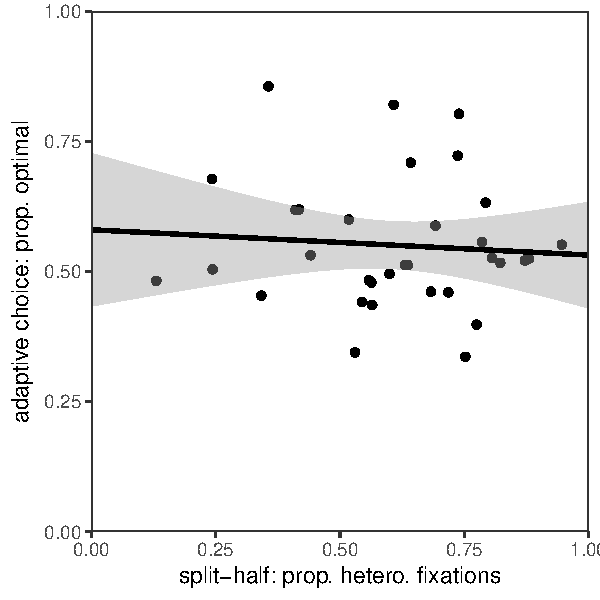
\includegraphics[width=3.25cm]{../Scripts/scratch/ls_v_ac_opt.pdf}}
% \subfigure[][]{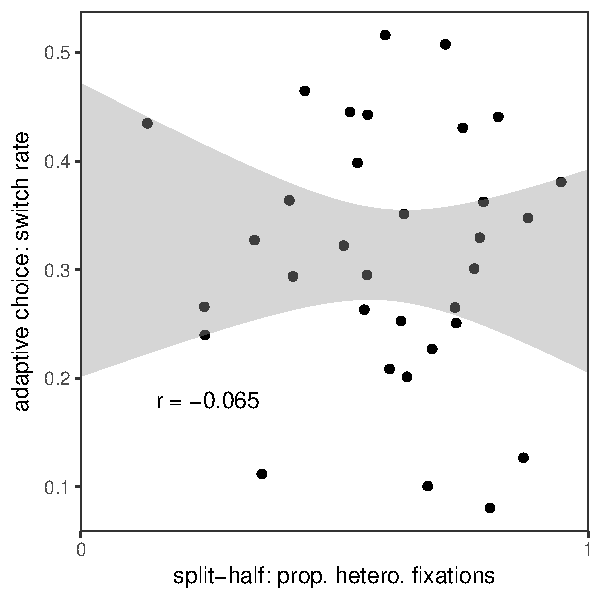
\includegraphics[width=3.25cm]{../Scripts/scratch/ls_v_ac_sr.pdf}}
% \subfigure[][]{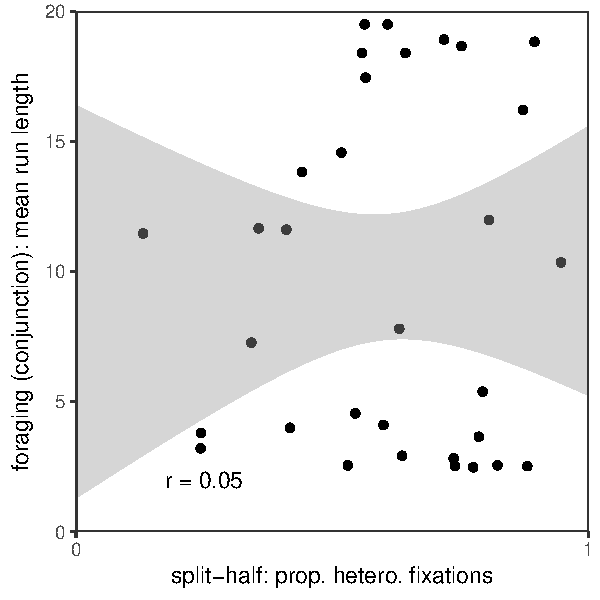
\includegraphics[width=3.25cm]{../Scripts/scratch/ls_v_fg_runlength.pdf}}
% \caption{Correlation between the optimal behaviour in the split-half and (a) adaptive choice paradigms; (b) average run length in the conjunction foraging paradigm; and (b) optimal behaviour in the adaptive choice paradigm and mean run length on the conjunction experiment.}
% \label{fig:between_para_rt}
% \end{figure}


\begin{figure}
\centering
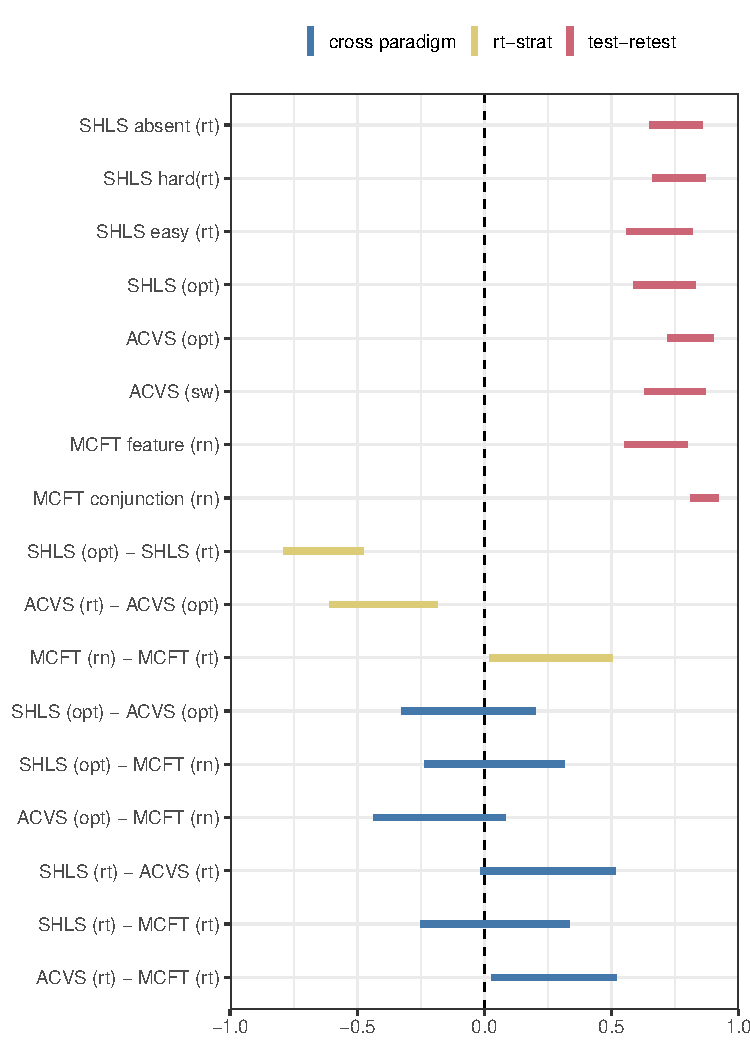
\includegraphics[width=6.5cm]{../Scripts/scratch/cor_comparison.pdf}
\caption{Lots of correlations!}
\label{fig:all_the_cor}
\end{figure}


%%%%%%%%%%%%%%%%%%%%%%%%%%%%%%%%%%%%%%%%%%%%%%%%%%%%%%%%%%%%%%%%%%%%%%%%%%%%%%%%%%%%
\section{Discussion}
%%%%%%%%%%%%%%%%%%%%%%%%%%%%%%%%%%%%%%%%%%%%%%%%%%%%%%%%%%%%%%%%%%%%%%%%%%%%%%%%%%%%

While we have successfully replicated the range of individual differences found in each of these studies, with a larger sample size than the original papers, the between-paradigm correlations give at most $R^2 = 0.1$, and this is a generous interpretation that would fail to pass the usual criteria for null hypothesis significance testing. Knowing how one person will behave in one of these paradigms apparently tells us very little about how they will perform in the others. This can be contrasted with the relatively high test-retest correlations of all three of the tasks individually, which range from [x to x]. 



I think he sees it as a positive thing that they tasks don't correlate, because it suggests they capture unique variation in behaviour glass half full approach 

Mention \cite{vogel2008}.
From \cite{proulx2011} - \textit{Vogel and colleagues have found that an individual's ability to remember a greater number of items using working memory is related to a filtering capacity in visual search that suppresses attentional capture by distracting visual information [10,11,12]. Behavioural work in visual search has extended this research to
demonstrate that working memory correlates only with top-down
visual search performance where task relevance is crucial, but not
with  bottom-up  visual  search  tasks  where  salience  in  the
environment guides attention \cite{sobel2007}}


Mention \cite{stoet2011}.


\bibliographystyle{plain}
\bibliography{literature}

\end{document}
